\section{Results}\label{sec:ciResults}

The direct result of the limit setting procedure is a limit on the number of signal events in the SR. Explicitly the claim is that the contribution from a non-background process to the number of expected events in the SR is \emph{less} than a given number, $N_\text{excl}$, with 95\% confidence. This means that signal models predicting \emph{more} than $N_\text{excl}$ in the SR is excluded with 95\% confidence. Limits on $N_\text{excl}$ can therefore be converted into limits on the contact interaction scale $\Lambda$ by considering the number of predicted signal events in the SR from a given $\Lambda$ model. The limits on $N_\text{excl}$ are described in section \ref{sec:limNSig} while the conversion of these to limits on $\Lambda$ is described in section \ref{sec:limLambda}.

\label{sec:Data}
\subsection{Data}

\begin{figure}[!htpb]
\centering
\subfloat[][]{{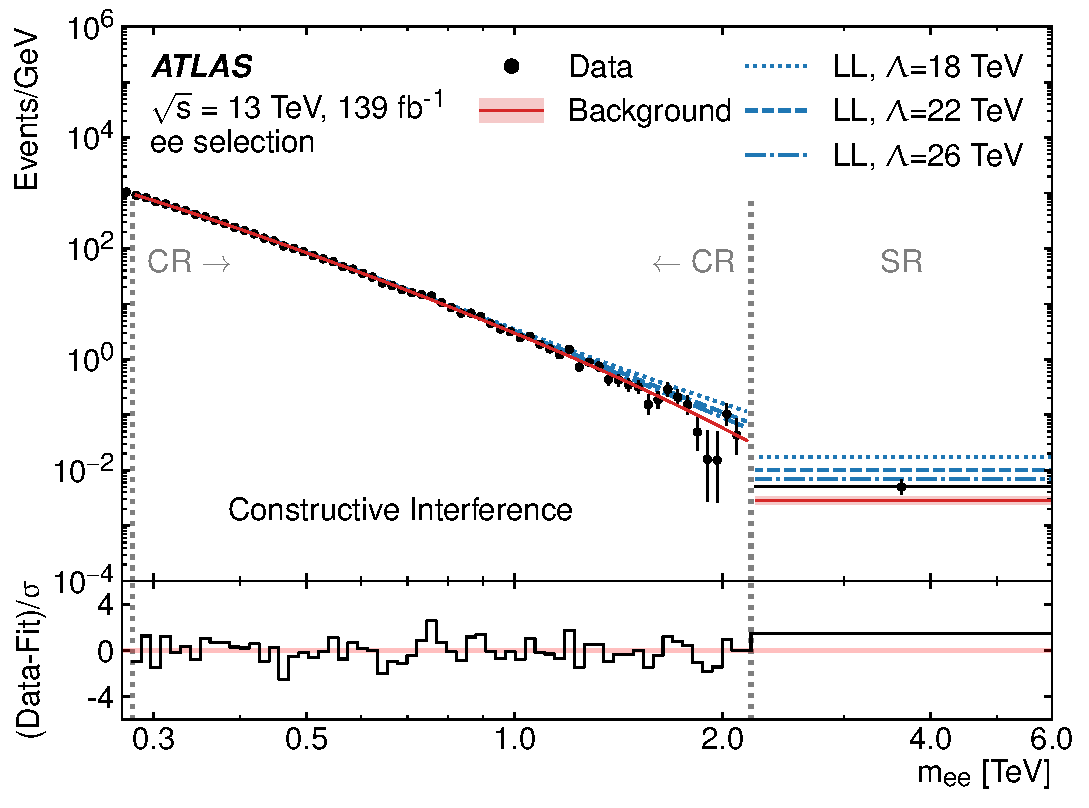
\includegraphics[width=0.5\textwidth]{figures/ci/results/fig_02a.pdf}}} % will be fig_02a.pdf
\subfloat[][]{{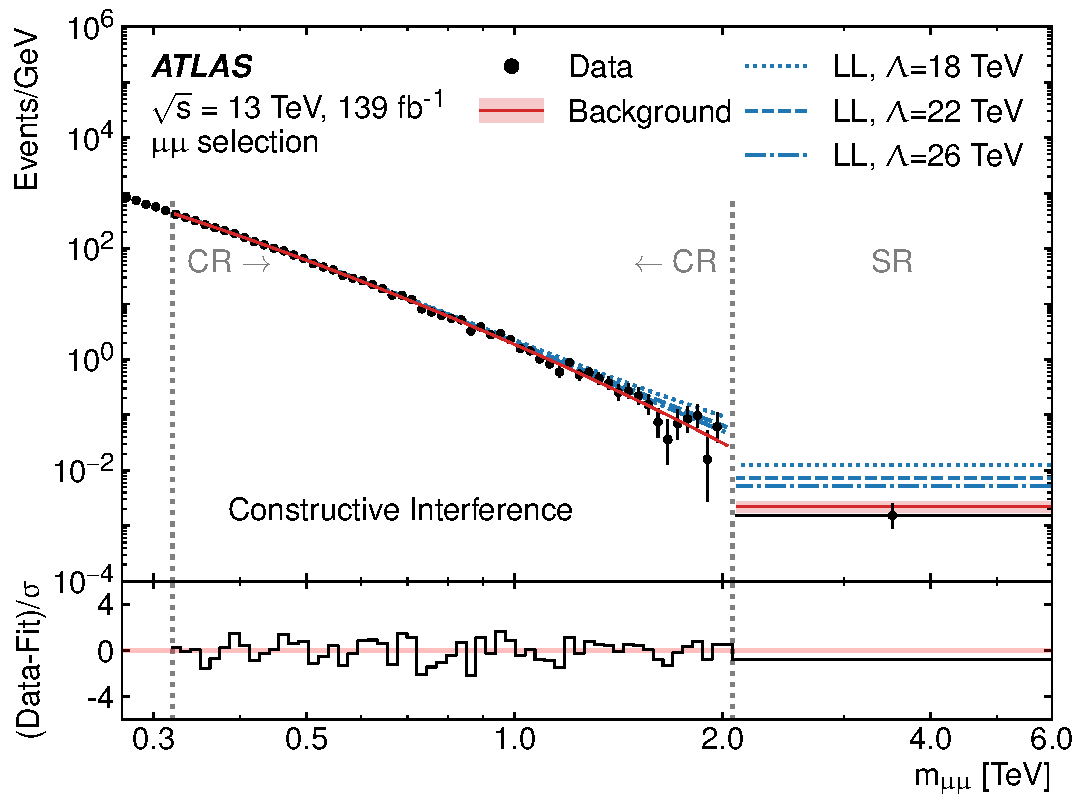
\includegraphics[width=0.5\textwidth]{figures/ci/results/fig_02b.pdf}}}\\ % will be fig_02b.pdf
\subfloat[][]{{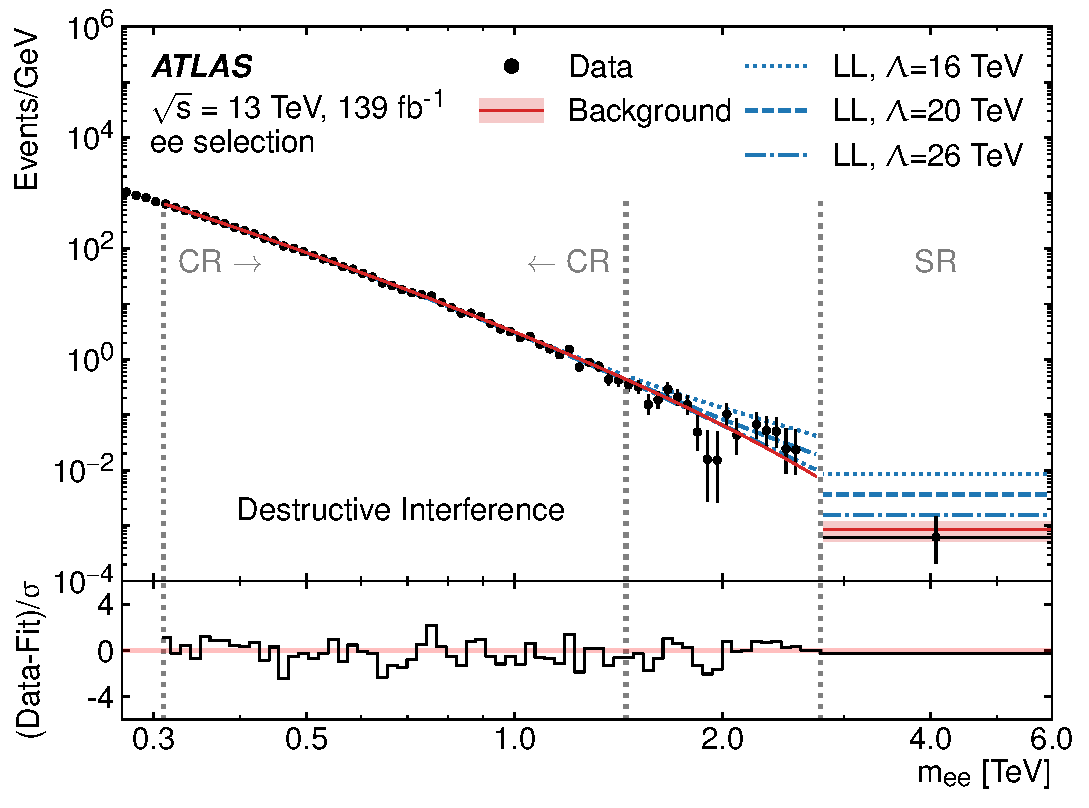
\includegraphics[width=0.5\textwidth]{figures/ci/results/fig_02c.pdf}}} % will be fig_02c.pdf
\subfloat[][]{{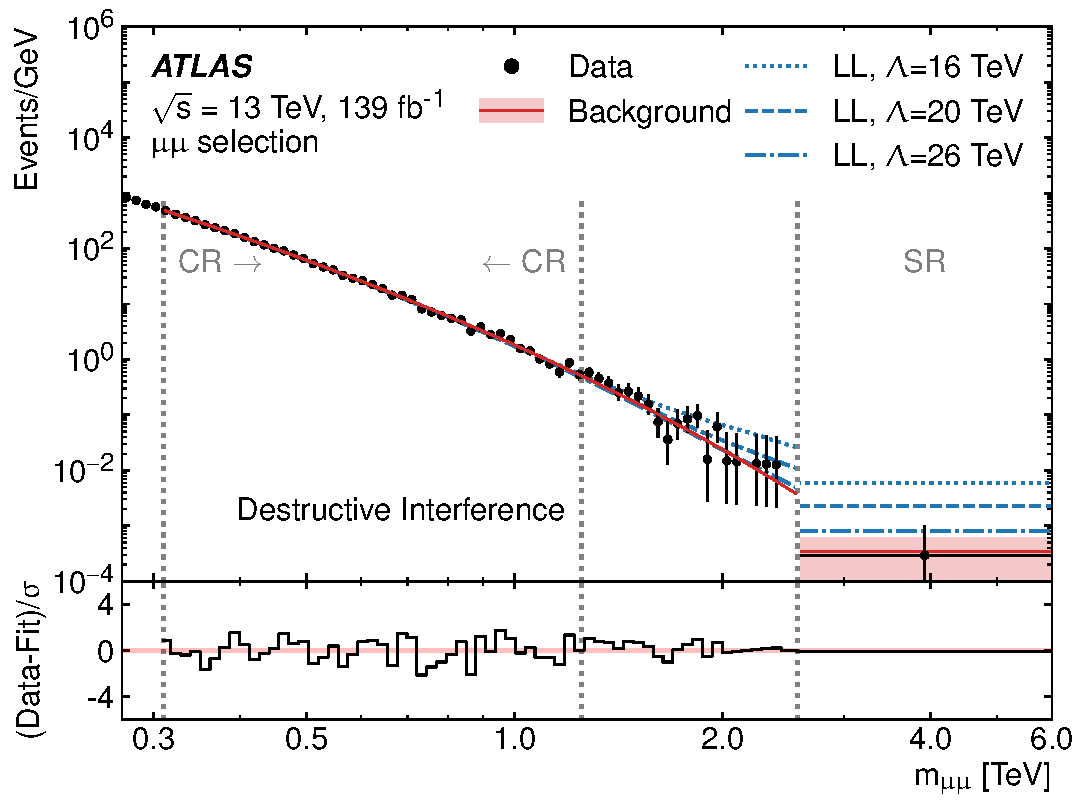
\includegraphics[width=0.5\textwidth]{figures/ci/results/fig_02d.pdf}}} % will be fig_02d.pdf
\caption{
Distributions of the invariant mass of dilepton pairs passing the full selection for dielectrons (left) and dimuons (right), and showing CR and SR for constructive interference (top) and destructive interference (bottom).
Figures (c) and (d) show the region between the SR and CR, but this is not used by the fit.
The data points are plotted at the centre of each bin as the number of events divided by the bin width, which is constant in $\log{(m_{\ell\ell})}$.
The error bars indicate statistical uncertainties only.
A few CI benchmark signal shapes are shown, scaled to the data luminosity and superimposed by subtracting the LO DY component and adding the resulting shape to the background shape obtained from the fit.
These signals have LL chirality with $\Lambda=$ 18, 22, and 26~TeV for the constructive case and $\Lambda=$16, 20, and $26$~TeV for the destructive case.
The background-only fit is shown in solid red, with the light red area being its uncertainty.
The boundaries of the CR and SR corresponding to the signals used are shown in dotted vertical lines for reference and marked by arrows.
%In the destructive interference case, the signal shapes do not differ much on the scale used for these plots.
The differences between the data and the fit results in units of standard deviations of the statistical uncertainty are shown in the bottom panels.
}
\label{fig:ciCiFits}
\end{figure}


\label{sec:Yields}
\subsection{Yields}

Table \ref{tab:yields} lists the expected yields for the background, with uncertainties and the observed yield in data for the different signal regions considered. The corresponding fits are shown in Subsection \ref{sec:dataFits}. The significance of a signal is summarised by a p-value, the probability of observing an excess at least as signal-like as the one observed in data, in the absence of signal. The p-value of the background-only hypothesis (p0) is determined from a profile-likelihood-ratio-test statistic in the frequentist method following \ref{sec:stats}, using 500000 toys and are summarised in Table \ref{tab:pVals}.

\begin{table}[htp]
    \centering
    \begin{tabular}{l | c c c c c c c c c c}
    \toprule
    % Signal Region & Background Exp & Observed data & Stat Unc of Fit & ISS & CRBU \\
    % ee - const           & 12.26 & 19 & 2.41 & 0.57 & 0.29 \\
    % ee - dest            & 2.73  & 2 & 1.66 & 0.35 & 0.02 \\
    % $\upmu\upmu$ - const & 9.60  & 6 & 2.05 & 0.46 & 0.18 \\
    % $\upmu\upmu$  - dest & 1.44  & 2 & 0.84 & 0.18 & 0.05 \\
    Channel & Interference & Expected & Observed & SU & ISSU & CRBU & Quad \\
    ee                & Constructive & 12.26 & 19 & 14.17\% & 4.37\% & 2.35\% & 15.02\% \\
    ee                & Destructive  & 2.73  & 2  & 34.30\% & 7.37\% & 0.49\% & 35.08\% \\
    $\upmu\upmu$      & Constructive & 9.60  & 6  & 21.31\% & 5.52\% & 1.88\% & 22.10\% \\
    $\upmu\upmu$      & Destructive  & 1.44  & 2  & 58.25\% & 24.32\% & 3.80\% & 63.24\% \\
    \bottomrule\end{tabular}
    \caption{Yields in the SR's for the data and from background fits with uncertainties.}
    \label{tab:yields}
    \end{table}

\begin{table}[htp]
    \centering
    \begin{tabular}{l   r r@{}l c }
    \toprule
    \multicolumn{1}{c}{SR} & Data & \multicolumn{2}{c}{Background} & Significance \\
    \midrule
    \ee   Const. & 19 & 12.4 & $\pm1.9$ & ~~~1.28 \\
    \ee   Dest.  & 2  & 3.1  & $\pm1.1$  & --~0.19 \\
    \midrule
    \mm Const. & 6  & 9.6  & $\pm2.1$  & --~0.99 \\
    \mm Dest.  & 1  & 1.4  & $\pm0.9$  & --~0.58 \\
    \bottomrule
    \end{tabular}
    \caption{The dielectron and dimuon event yields for the data, the expected background and the respective significance in the different SRs used in the analysis.  The p-value of each observation is defined as the probability, given the background-only hypothesis, of an observation at least as large as that seen in the data.  The significance is the Gaussian cumulative density function of the p-value, and negative significances correspond to deficits. }
    \label{tab:pVals}
\end{table}

\subsection{Limits on signal events}
\label{sec:limNSig}

The limits in this section are set on the number of signal events, $N_\text{excl}$, in a high-mass signal region. Physical processes not described by the background model with yields in the SR above $N_\text{excl}$ are excluded with a confidence level of 95\%.

For some signal models, the question as to whether the process is ``not described by the background model'' may be unclear. The background model is determined for processes contributing to the yields in the corresponding control region. A model which predicts no contribution in the CR, and a contribution to the SR above $N_\text{excl}$ may be considered excluded. For models which do predict a contribution to the CR and that contribution is assumed to be negligible: this assumption needs to be tested before reinterpreting these limits. The test employed by this analysis for the contact interaction models is described in section \ref{sec:bootstrappingBkg}.

Table \ref{tab:yields_sig} shows the 95\% CL limits on the number of signal events in the SR for the muon channel, electron channel, and dilepton combination. In addition, the upper limit on the visible cross section times branching fraction $(\sigma_\textrm{vis}\times\textrm{Br})$ along with the efficiencies and yields for a number of CI models.  The Upper limits are evaluated with the modified frequentist CLS method using 400000 toys.

% \begin{table}[htp]
% \centering
% \begin{tabular}{l r r r r r r}\toprule
% Channel & Expected & Observed & $+1\sigma$ & $-1\sigma$\\
% mm-const & 6.91 & 4.72 & 10.66 & 4.49\\
% ee-const & 17.06 & 23.68 & 22.58 & 13.32\\
% mm-dest & 3.95 & 3.61 & 6.32 & 2.53\\
% ee-dest & 4.98 & 2.94 & 8.02 & 3.09\\
% \bottomrule\end{tabular}
% \caption{Observed and expected limits on the number of signal events to 95\% CL. }
% \label{tab:nSigLimits}
% \end{table}

% \begin{table}[htp]
% \centering
% \begin{tabular}{r l l l l l l l l l}\toprule
% Channel & Expected & Observed & $+1\sigma$ & $-1\sigma$ \\
% mm-const & 6.88 & 5.37 & 10.62 & 4.47\\
% ee-const & 11.95 & 16.31 & 16.46 & 8.97\\
% mm-dest & 3.77 & 3.46 & 6.09 & 2.41\\
% ee-dest & 4.92 & 4.62 & 7.63 & 3.24\\
% \bottomrule\end{tabular}
% \caption{Observed and expected limits on the number of signal events to 95\% CL. }
% \label{tab:nSigLimits}
% \end{table}

% \begin{table}[htp]
% \centering
% \begin{tabular}{r c c c c c c c c c c c}\toprule
% & & & LL $\sigma\times\text{B}$ [fb] \\
% \midrule
% \multirow{2}{*}[-1.5em]{\begin{sideways}Const\end{sideways}} & \multirow{2}{*}{$ee$} & Expected & 0.0712 \\
% & & Observed & 0.1155 \\
% \cmidrule{2-4}
%  & \multirow{2}{*}{$\mu\mu$} & Expected & 0.0575 \\
% & & Observed & 0.0408 \\
% \cmidrule{2-4}
% \multirow{2}{*}[-1.5em]{\begin{sideways}Dest\end{sideways}} & \multirow{2}{*}{$ee$} & Expected & 0.0382 \\
% & & Observed & 0.0341 \\
% \cmidrule{2-4}
%  & \multirow{2}{*}{$\mu\mu$} & Expected & 0.0282 \\
% & & Observed & 0.0253 \\
% \cmidrule{2-4}
% \bottomrule\end{tabular}
% \caption{Observed and expected limits on the number of visible cross section times branching ratio in each signal region, set at 95\% CL. {\color{red} Will be updated with final values soon}}
% \label{tab:xsBrLimits}
% \end{table}

% \begin{table}[htp]
%     \begin{center}
%     \caption{The observed model-independent upper limit on the visible cross section times branching fraction $(\sigma_\textrm{vis}\times\textrm{Br})$ and the number of signal events $(N_\textrm{sig})$ in the dielectron and dimuon SRs used in the analysis. The yields for few CI signal points (LL only) are listed along with the signal efficiencies for reference.}
%     {\footnotesize
%     \begin{tabular}{l | c | c c | c c c c c c}
%         \toprule
%         SR           & Limit on $\sigma_\textrm{vis}\times\textrm{Br}$ [fb] & \multicolumn{2}{c|}{Limit on $N_\textrm{sig}$} & \multicolumn{6}{c}{Signal (LL only)} \\
%                      &         &  &       & \multicolumn{2}{c}{$\Lambda=20~\TeV$} & \multicolumn{2}{c}{$\Lambda=30~\TeV$}  & \multicolumn{2}{c}{$\Lambda=40~\TeV$} \\
%                      &         & Exp. & Obs.      & $N_\textrm{s}$ & $\epsilon_\textrm{s}$~[\%] & $N_\textrm{s}$ & $\epsilon_\textrm{s}$~[\%] & $N_\textrm{s}$ & $\epsilon_\textrm{s}$~[\%] \\
%         \hline
%         \mm Const. & 0.042   & 8.0 & 5.8   & 16.5 & 43 & 4.5 & 43 & 1.9 & 43 \\ % \mm Const.
%         \mm Dest.  & 0.027   & 4.0 & 3.8   & 4.1 & 43 & 0.3 & 42 & -0.1 & 44 \\ % \mm Dest.
%         \hline
%         \ee   Const. & 0.117   & 10.0 & 16.3  & 22.7 & 69 & 6.0 & 69 & 2.6 & 69 \\ % \ee   Const.
%         \ee   Dest.  & 0.038   & 5.4  & 5.4   & 5.5 & 70 & 0.6 & 70 & -0.1 & 69 \\ % \ee   Dest.
%         \bottomrule
%         \end{tabular}
%     }
%     \label{tab:yields_sig}
%     \end{center}
% \end{table}

\begin{table}[htp]
\begin{center}
\caption{The observed model-independent upper limit at 95\% CL on the visible cross-section times branching fraction $(\sigma_\textrm{vis}\times\mathcal{B})$ and the number of signal events $(N_\textrm{sig})$ in the dielectron and dimuon SRs used in the analysis. The expected yields for a few CI signal points (LL chirality only) are listed along with the signal acceptance times efficiency $(\mathcal{A}\times\epsilon_\textrm{sig})$ values for reference.}
{\scriptsize
\begin{tabular}{l | c c | c d{1} | d{1} c d{1} c d{1} c}
% \Xhline{2\arrayrulewidth}
\toprule
\multicolumn{1}{c|}{\multirow{3}{*}{SR}}           & \multicolumn{2}{c|}{Limit on $\sigma_\textrm{vis}\times\mathcal{B}$ [fb]} & \multicolumn{2}{c|}{Limit on $N_\textrm{sig}$} & \multicolumn{6}{c}{Signal (LL chirality only)} \\
             &  \multirow{2}{*}{Exp.} & \multirow{2}{*}{Obs.}  & \multirow{2}{*}{Exp.} & \multicolumn{1}{r|}{\multirow{2}{*}{Obs.}} & \multicolumn{2}{c}{$\Lambda=20~$TeV} & \multicolumn{2}{c}{$\Lambda=30~$TeV}  & \multicolumn{2}{c}{$\Lambda=40~$TeV} \\
             % &  Exp.   & Obs.  & Exp. & \multicolumn{1}{r|}{Obs.} & N_\text{sig} & $\mathcal{A}\times\epsilon_\text{sig}$~[\%] & N_\text{sig} & $\mathcal{A}\times\epsilon_\text{sig}$~[\%] & N_\text{sig} & $\mathcal{A}\times\epsilon_\text{sig}$~[\%] \\
             &     & & &  & N_\text{sig} & $\mathcal{A}\times\epsilon_\text{sig}$~[\%] & N_\text{sig} & $\mathcal{A}\times\epsilon_\text{sig}$~[\%] & N_\text{sig} & $\mathcal{A}\times\epsilon_\text{sig}$~[\%] \\
\midrule
\ee   Const. & 0.067   & 0.115 & 9.3  & 16.0 & 39.1 & 69  & 10.3 & 69  &  4.4  & 69 \\
\ee   Dest.  & 0.036   & 0.032 & 5.0  & 4.4  & 9.6  & 70  & 1.0  & 70  & -0.1 & 69 \\
\midrule
\mm Const. & 0.057   & 0.042 & 8.0 & 5.8   & 28.5 & 43  & 7.7  & 43  &  3.4  & 43 \\
\mm Dest.  & 0.029   & 0.027 & 4.0 & 3.8   & 7.1  & 43  & 0.6 & 42  & -0.2 & 44 \\
% \Xhline{2\arrayrulewidth}
\bottomrule
\end{tabular}
}
\label{tab:yields_sig}
\end{center}
\end{table}


% \begin{table}[htp]
% \centering
% \begin{tabular}{l r r r r r r}\toprule
% & & LL $\Lambda$ TeV & LR $\Lambda$ TeV & RL $\Lambda$ TeV & RR $\Lambda$ TeV \\
% \multirow{3}{*}{mm-const} & Expected & 31.27 & 28.84 & 28.66 & 31.07\\
% & $+1\sigma$ & 27.17 & 25.44 & 25.32 & 27.03\\
% & $-1\sigma$ & 36.19 & 32.80 & 32.55 & 35.89\\
% \hline
% \multirow{3}{*}{ee-const} & Expected & 28.23 & 26.37 & 26.22 & 28.06\\
% & $+1\sigma$ & 25.83 & 24.34 & 24.22 & 25.72\\
% & $-1\sigma$ & 30.64 & 28.34 & 28.15 & 30.44\\
% \hline
% \multirow{3}{*}{mm-dest} & Expected & 22.61 & 24.19 & 24.21 & 22.83\\
% & $+1\sigma$ & 20.69 & 21.81 & 21.82 & 20.84\\
% & $-1\sigma$ & 24.44 & 26.66 & 26.69 & 24.74\\
% \hline
% \multirow{3}{*}{ee-dest} & Expected & 22.97 & 24.43 & 24.40 & 23.18\\
% & $+1\sigma$ & 20.90 & 21.89 & 21.88 & 21.06\\
% & $-1\sigma$ & 25.11 & 27.17 & 27.14 & 25.38\\
% \bottomrule\end{tabular}
% \caption{Upper and lower bounds for each limit. }
% \label{tab:nSigLimits}
% \end{table}


\subsection{Limits on $\Lambda$}
\label{sec:limLambda}

In this section the limits from section \ref{sec:limNSig} are reinterpreted as limits on the contact interaction scale $\Lambda$. Using the procedure described in section \ref{sec:signalLimitConversion}, the limits on the number of signal events are converted to limits on the CI scale $\Lambda$. Table \ref{tab:lambdaLimits1} gives the $\Lambda$ up to which contact interactions are excluded with a CL of 95\% for the muon channel, electron channel, and dilepton combination. Comparison of limits set on $\Lambda$ directly and re-interpreted limits from the limits on signal events are shown in Appendix \ref{sec:nSigVsLambda}.

\begin{table}[htp]
\begin{center}
\caption{Expected and observed lower limits at 95$\%$ CL on $\Lambda$ in TeV for the dielectron and dimuon channels separately and the combined dilepton channel and for CI signal hypotheses with constructive and destructive interference and different chiralities.}
{\begin{tabular}{c c c c c c c c c c c c}\toprule
Int. & Channel & Exp./Obs. & LL & LR & RL & RR \\
\midrule
\multirow{3}{*}[-1.5em]{\begin{sideways}Constructive\end{sideways}} & \multirow{2}{*}{$ee$} & Expected & 31.1 & 28.9 & 28.7 & 30.9 \\
& & Observed & 26.1 & 24.7 & 24.6 & 26.0 \\
\cmidrule{2-7}
 & \multirow{2}{*}{$\mu\mu$} & Expected & 29.2 & 27.1 & 27.0 & 29.0 \\
& & Observed & 32.7 & 30.0 & 29.8 & 32.6 \\
\cmidrule{2-7}
 & \multirow{2}{*}{$\ell\ell$} & Expected & 37.6 & 34.0 & 33.7 & 37.3 \\
& & Observed & 35.8 & 32.5 & 32.3 & 35.5 \\
\midrule
\multirow{3}{*}[-1.5em]{\begin{sideways}Destructive\end{sideways}} & \multirow{2}{*}{$ee$} & Expected & 23.0 & 24.4 & 24.4 & 23.2 \\
& & Observed & 23.5 & 25.1 & 25.1 & 23.7 \\
\cmidrule{2-7}
 & \multirow{2}{*}{$\mu\mu$} & Expected & 22.0 & 23.6 & 23.6 & 22.2 \\
& & Observed & 22.3 & 23.9 & 23.9 & 22.5 \\
\cmidrule{2-7}
 & \multirow{2}{*}{$\ell\ell$} & Expected & 25.6 & 28.0 & 28.0 & 25.9 \\
& & Observed & 26.0 & 28.8 & 28.8 & 26.5 \\
\bottomrule\end{tabular}}
\label{tab:lambdaLimits1}
\end{center}
\end{table}


\subsubsection{Additional signal models}
\label{sec:addlSigModels}

The limits shown in table \ref{tab:lambdaLimits1} are set without theoretical uncertainty on the signal model. This choice is made since we define out signal model, and consequently there is no uncertainty related to that definition. Additionally we set limits on other signal models, corresponding to other possible theoretical variations. These are shown for $1\sigma$ theoretical upwards (table \ref{tab:limits_on_lambda_theoryUp}) and downward (table \ref{tab:limits_on_lambda_theoryDn}) variations on the signal strength.

\begin{table}[htp]
\begin{center}
\caption{Expected and observed lower limits at 95$\%$ CL on $\Lambda$ in TeV for the dielectron and dimuon channels separately
and for the combined electron-muon channel, for a theoretical variation on the CI signal hypotheses with constructive
and destructive interference and different chiralities.
The CI signal hypothesis has been increased by $+1\sigma_\text{s}^\text{Theory}$.}
{\begin{tabular}{r c c c c c c c c c c c}\toprule
Int. & Channel & Exp./Obs. & LL & LR & RL & RR \\
\midrule
\multirow{3}{*}[-1.5em]{\begin{sideways}Constructive\end{sideways}} & \multirow{2}{*}{$ee$} & Expected & 31.9 & 29.4 & 29.4 & 31.7 \\
& & Observed & 26.8 & 25.2 & 25.2 & 26.6 \\
\cmidrule{2-7}
 & \multirow{2}{*}{$\mu\mu$} & Expected & 31.1 & 28.8 & 28.6 & 30.9 \\
& & Observed & 35.1 & 31.8 & 31.6 & 34.7 \\
\cmidrule{2-7}
 & \multirow{2}{*}{$\ell\ell$} & Expected & 39.6 & 35.6 & 35.4 & 39.3 \\
& & Observed & 38.6 & 34.7 & 34.4 & 38.2 \\
\midrule
\multirow{3}{*}[-1.5em]{\begin{sideways}Destructive\end{sideways}} & \multirow{2}{*}{$ee$} & Expected & 23.3 & 24.9 & 24.9 & 23.5 \\
& & Observed & 23.8 & 25.5 & 25.5 & 24.0 \\
\cmidrule{2-7}
 & \multirow{2}{*}{$\mu\mu$} & Expected & 23.2 & 25.2 & 25.1 & 23.5 \\
& & Observed & 23.5 & 25.4 & 25.4 & 23.7 \\
\cmidrule{2-7}
 & \multirow{2}{*}{$\ell\ell$} & Expected & 26.5 & 29.2 & 29.2 & 26.9 \\
& & Observed & 26.9 & 29.9 & 29.9 & 27.3 \\
\bottomrule\end{tabular}}\\
\label{tab:limits_on_lambda_theoryUp}
\end{center}
\end{table}

\begin{table}[htp]
\begin{center}
\caption{Expected and observed lower limits at 95$\%$ CL on $\Lambda$ in TeV for the dielectron and dimuon channels separately
and for the combined electron-muon channel, for a theoretical variation on the CI signal hypotheses with
constructive and destructive interference and different chiralities.
The CI signal hypothesis has been reduced by $-1\sigma_\text{s}^\text{Theory}$.}
{\begin{tabular}{r c c c c c c c c c c c}\toprule
Int. & Channel & Exp./Obs. & LL & LR & RL & RR \\
\midrule
\multirow{3}{*}[-1.5em]{\begin{sideways}Constructive\end{sideways}} & \multirow{2}{*}{$ee$} & Expected & 30.3 & 28.1 & 28.0 & 30.0 \\
& & Observed & 25.5 & 24.0 & 24.0 & 25.3 \\
\cmidrule{2-7}
 & \multirow{2}{*}{$\mu\mu$} & Expected & 26.7 & 25.1 & 25.0 & 26.6 \\
& & Observed & 30.3 & 27.9 & 27.7 & 30.0 \\
\cmidrule{2-7}
 & \multirow{2}{*}{$\ell\ell$} & Expected & 35.4 & 32.1 & 31.9 & 35.0 \\
& & Observed & 32.7 & 30.1 & 30.0 & 32.5 \\
\midrule
\multirow{3}{*}[-1.5em]{\begin{sideways}Destructive\end{sideways}} & \multirow{2}{*}{$ee$} & Expected & 22.5 & 23.9 & 23.9 & 22.7 \\
& & Observed & 23.0 & 24.5 & 24.5 & 23.3 \\
\cmidrule{2-7}
 & \multirow{2}{*}{$\mu\mu$} & Expected & 18.7 & 18.3 & 18.3 & 18.7 \\
& & Observed & 20.7 & 21.8 & 21.7 & 20.8 \\
\cmidrule{2-7}
 & \multirow{2}{*}{$\ell\ell$} & Expected & 24.5 & 26.5 & 26.5 & 24.8 \\
& & Observed & 25.1 & 27.4 & 27.4 & 25.4 \\
\bottomrule\end{tabular}} \\
\label{tab:limits_on_lambda_theoryDn}
\end{center}
\end{table}

\clearpage

\subsection{Exclusion plots for number of signal events}

Limits on the number of signal events for each signal region considered is shown in figure~\ref{fig:ciCiLimNSig} .

\begin{figure}[htb!]
\begin{center}
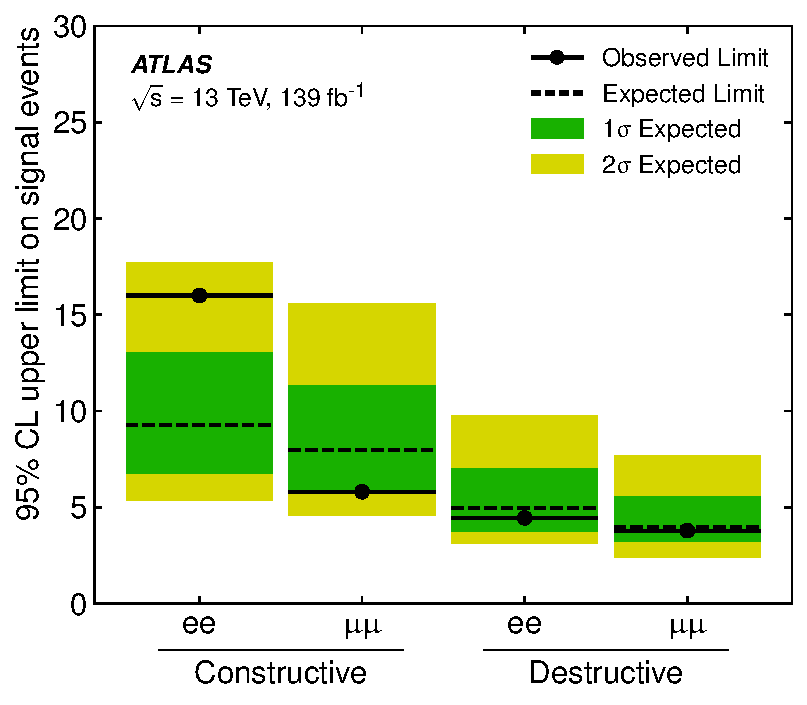
\includegraphics[width=0.5\linewidth]{figures/ci/results/fig_03a.pdf}
\end{center}
\vspace{-.4cm}
\caption{Limits on the number of signal events in the respective signal region for each model. }
\label{fig:ciCiLimNSig}
\end{figure}

\subsection{Exclusion plots for $\Lambda$}
Limit on the CI energy scale $\Lambda$ for the different chiral and interference models for the dielectron channel shown in figure~\ref{fig:ciCiEeLimLambda}, dimuon channel shown in figure~\ref{fig:ciCiMmLimLambda} and combined channel shown in figure~\ref{fig:ciCiLlLimLambda}.

\begin{figure}[htb]
\begin{center}
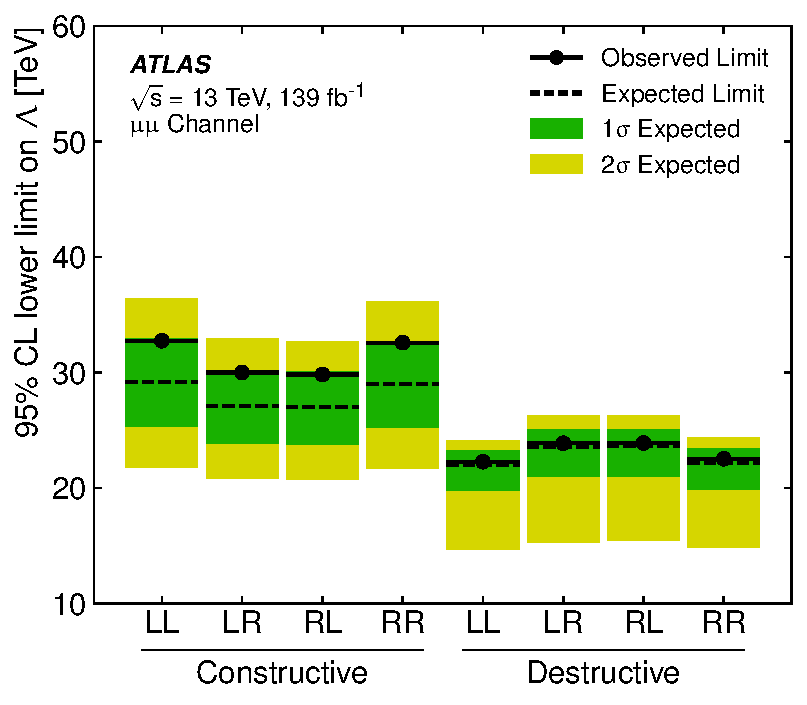
\includegraphics[width=0.5\linewidth]{figures/ci/results/fig_04a.pdf}
\end{center}
\vspace{-.4cm}
\caption{Limits on the contact interaction scale $\Lambda$ for the muon channel for each interference and chiral model shown in the bottom axis, the expected and observed limits are shown. The dotted line shows the expected limits and the green and yellow error bars show the 1 and $2\sigma$ uncertainty bands on the expectation. The black points show the observed limits.}
\label{fig:ciCiMmLimLambda}
\end{figure}

\begin{figure}[htb]
\begin{center}
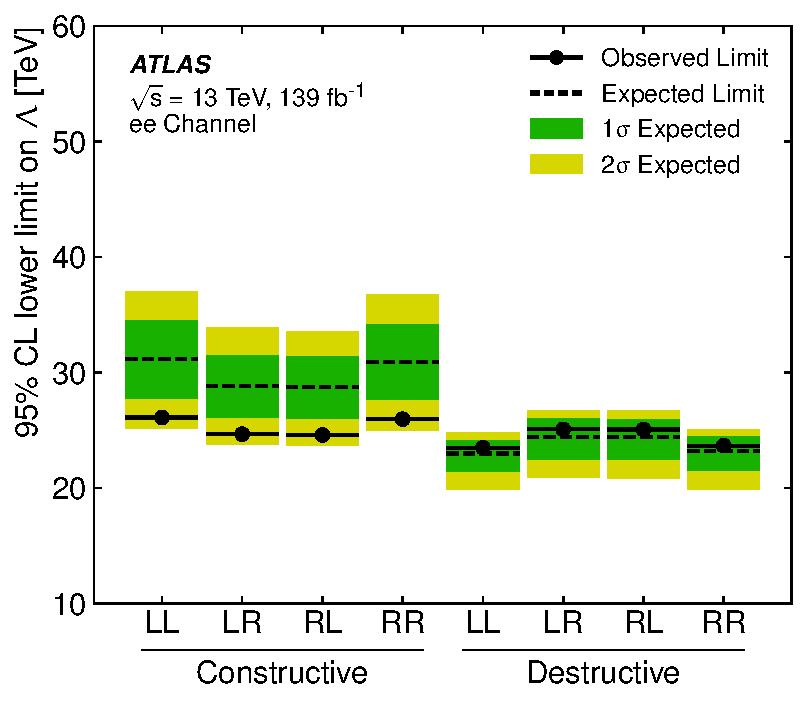
\includegraphics[width=0.5\linewidth]{figures/ci/results/fig_04b.pdf}
\end{center}
\vspace{-.4cm}
\caption{Limits on the contact interaction scale $\Lambda$ for the electron channel for each interference and chiral model shown in the bottom axis, the expected and observed limits are shown. The dotted line shows the expected limits and the green and yellow error bars show the 1 and $2\sigma$ uncertainty bands on the expectation. The black points show the observed limits.}
\label{fig:ciCiEeLimLambda}
\end{figure}

\begin{figure}[htb]
    \begin{center}
    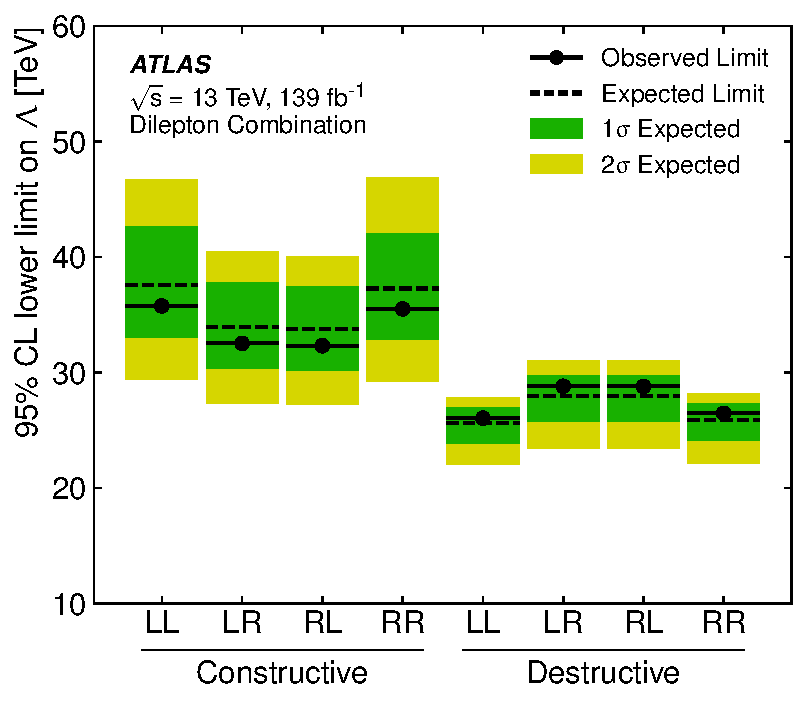
\includegraphics[width=0.5\linewidth]{figures/ci/results/fig_04c.pdf}
    \end{center}
    \vspace{-.4cm}
    \caption{Limits on the contact interaction scale $\Lambda$ for the combined channel for each interference and chiral model shown in the bottom axis, the expected and observed limits are shown. The dotted line shows the expected limits and the green and yellow error bars show the 1 and $2\sigma$ uncertainty bands on the expectation. The black points show the observed limits.}
    \label{fig:ciCiLlLimLambda}
\end{figure}

\begin{figure}[!htpb]
\centering
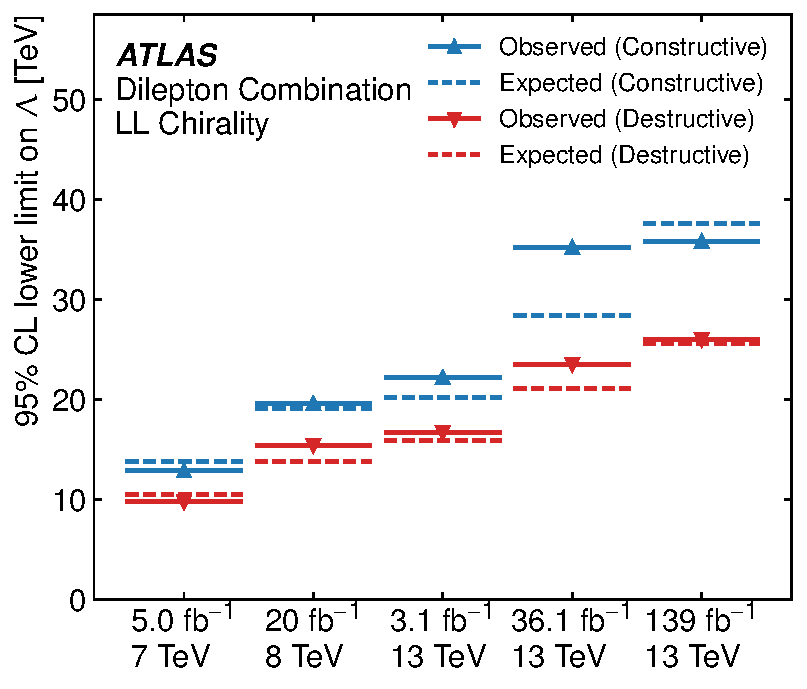
\includegraphics[width=0.70\textwidth]{figures/ci/results/figaux_05.pdf}
\caption{Comparison of the $\ell\ell$ constructive (blue) and destructive (red) LL chirality limits with previous ATLAS results. For results with Bayesian limits, the $\Lambda^{-4}$ prior is used. ($\sqrt{s}=13$~TeV 36.1 fb$^{-1}$ result: \cite{EXOT-2016-05}, $\sqrt{s}=13$~TeV 3.1 fb$^{-1}$ result: \cite{EXOT-2015-07}, $\sqrt{s}=8$~TeV 20 fb$^{-1}$ result: \cite{EXOT-2013-19}, $\sqrt{s}=7$~TeV 5.0 fb$^{-1}$ result: \cite{EXOT-2012-17}.)}
\label{fig:ciCiHistoricalLimits}
\end{figure}


\subsection{Fit and Signal Plots}

These plots show illustrations of the fitted background shape, along with some representative signal shapes. The parameters of the fitted background shape are given in table \ref{tab:fitpars}.

% server fit numbers (used for limit setting)
\begin{table}[htp]
\centering
\caption{Parameters for the functional form given in Eq.~(\ref{eq:b}). The uncertainties are statistical only.}
{\footnotesize
 \begin{tabular}{l  r@{}c@{}l r@{}c@{}l  r@{}c@{}l r@{}c@{}l }
\toprule
Parameter  &  \multicolumn{3}{c}{\ee, Constructive} &  \multicolumn{3}{c}{\ee, Destructive} &  \multicolumn{3}{c}{\mm, Constructive} &  \multicolumn{3}{c}{\mm, Destructive} \\
\midrule
 a         & \multicolumn{3}{c}{$(6.17 \pm 0.02)\times 10^\text{-3}$} & \multicolumn{3}{c}{$(7.87\pm 0.03)\times 10^\text{-3}$} & \multicolumn{3}{c}{$(6.90\pm 0.03)\times 10^\text{-6}$} & \multicolumn{3}{c}{$(4.39\pm 0.02)\times 10^\text{-7}$} \\
 b (fixed) & \multicolumn{3}{c}{6.1} & \multicolumn{3}{c}{6.1} & \multicolumn{3}{c}{1.3} & \multicolumn{3}{c}{1.3} \\
 c (fixed) & \multicolumn{3}{c}{1/2} & \multicolumn{3}{c}{1/2} & \multicolumn{3}{c}{1/3} & \multicolumn{3}{c}{1/3} \\
 $p_0$ &  ~~~~-12.2   & $\pm$ & 0.1       & ~~~~~-12.1  &$\pm$& 0.1   & ~~~~~-14.9  &$\pm$& 0.2   & ~~~~~-17.0 &$\pm$& 0.2 \\
 $p_1$ &  ~~~~-4.14   & $\pm$ & 0.02      & ~~~~~-4.16  &$\pm$& 0.03  & ~~~~~-4.42 &$\pm$& 0.04  &  ~~~~~-4.70 &$\pm$& 0.04 \\
 $p_2$ &  ~~~~-0.948  & $\pm$ & 0.005     & ~~~~~-0.945 &$\pm$& 0.006 & ~~~~~-0.927 &$\pm$& 0.008 & ~~~~~-0.846 &$\pm$& 0.008 \\
 $p_3$ &  ~~~~-0.0840 & $\pm$ & 0.0008    & ~~~~~-0.082 &$\pm$& 0.001 & ~~~~~-0.081 &$\pm$& 0.001 & ~~~~~-0.064 &$\pm$& 0.001 \\
\bottomrule\end{tabular}}
\label{tab:fitpars}
\end{table}

\subsection{Comparison with simulation}

Table \ref{tab:mcVsFit} shows a comparison, integrated in the corresponding signal region, between our fitted background estimate and the one derived from simulation. This table shows reasonable compatibility between the MC and the fit. A further comparison is made in figure \ref{fig:ciCiFitVsMc} shows a comparison between the fitted background estimate, and the MC. Here, the fitted background estimate is produced using the fit to data. Since we do not have shape based systematic uncertainties on the fit, only the shape itself is shown.

\begin{table}[htp]
\centering
\caption{Comparison between the background estimate in the SR, as derived from fitting the data ($N_\text{fit}$), and the estimation from simulated background ($N_\text{sim}$). The yields observed in data ($N_\text{obs}$) are also given. All systematic uncertainties are included.}
\begin{tabular}{l | r r r }\toprule
SR & $N_\text{sim}\pm\sigma_\text{sim}$ & $N_\text{fit}\pm\sigma_\text{fit}$ & $N_\text{obs}$ \\
\hline
\ee const.   & $13.3  \pm 1.9$  & $12.4 \pm 1.9$ & 19 \\
\ee dest.    & $2.9   \pm 0.6$  & $3.1  \pm 1.1$ & 2  \\ % fixed ee
\mm const. & $11.9  \pm 2.8$  & $9.6  \pm 2.1$ & 6  \\
\mm dest.  & $3.3   \pm 1.0$  & $1.4  \pm 0.9$ & 1  \\
\bottomrule\end{tabular}\\ %remember cline{1-2}
\label{tab:mcVsFit}
\end{table}


\begin{figure}[!htpb]
\centering
\subfloat[][]{{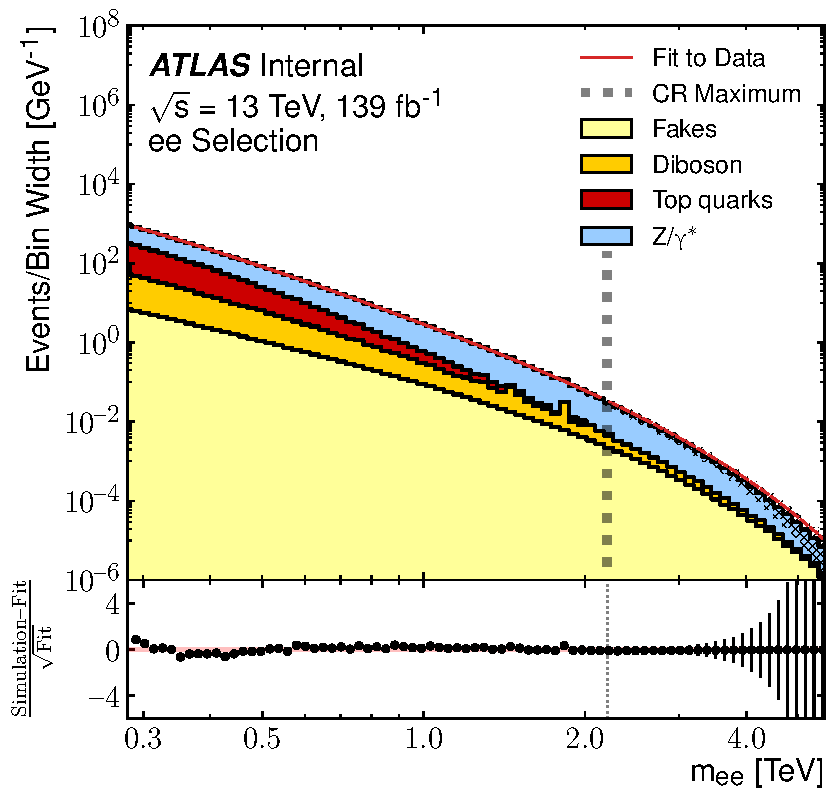
\includegraphics[width=0.45\textwidth]{figures/ci/results/figaux_08a.pdf}}}
\subfloat[][]{{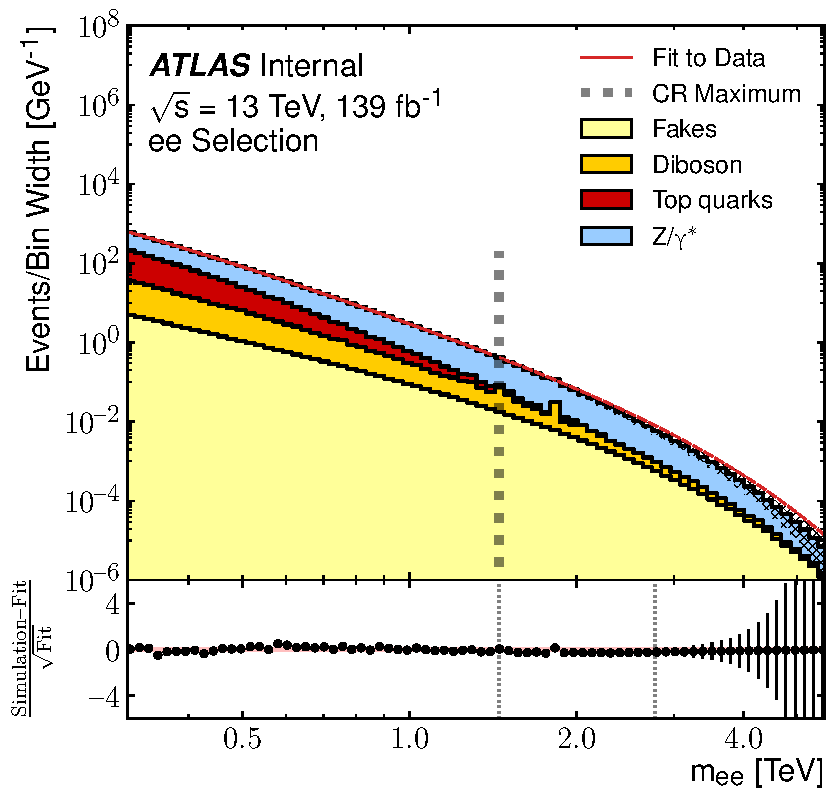
\includegraphics[width=0.45\textwidth]{figures/ci/results/figaux_08b.pdf}}} \\
\subfloat[][]{{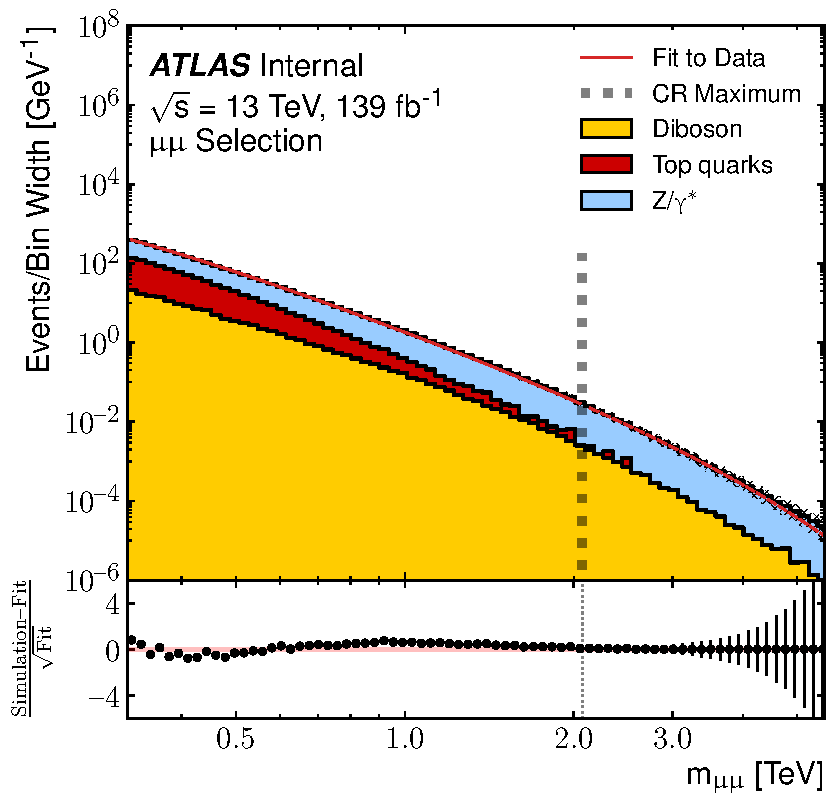
\includegraphics[width=0.45\textwidth]{figures/ci/results/figaux_08c.pdf}}}
\subfloat[][]{{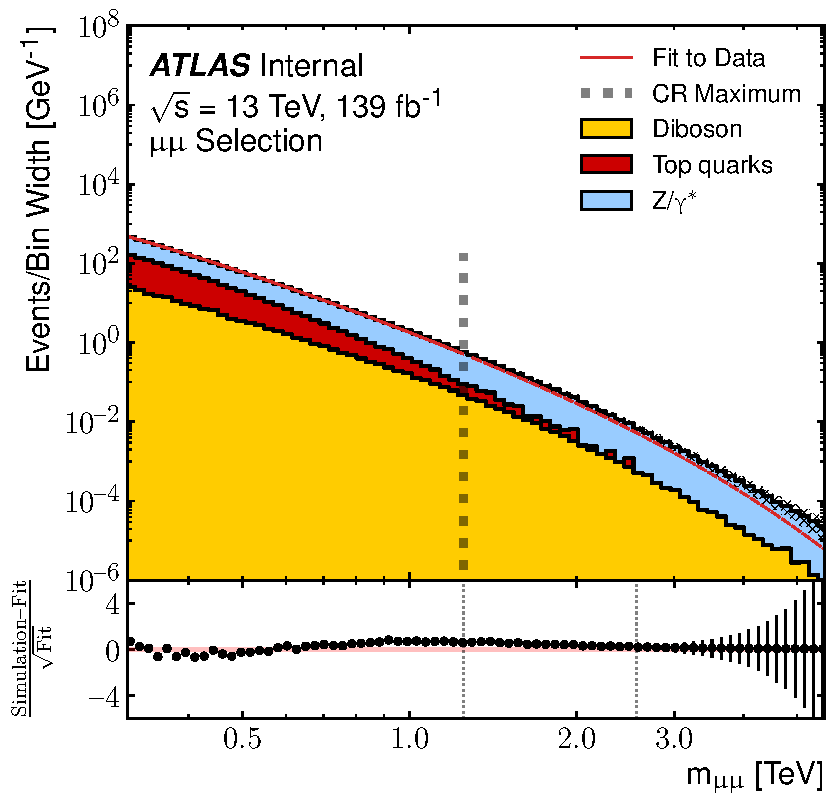
\includegraphics[width=0.45\textwidth]{figures/ci/results/figaux_08d.pdf}}}
\caption{Fits performed on data (red) are compared to the background simulation. The background simulation is used only to study performance and systematics. The uncertainties on the background simulation are theory only, and are provided as a rough estimate.
Shown for \ee constructive (a), \ee destructive (b), \mm constructive (c), and \mm destructive (d).}
\label{fig:ciCiFitVsMc}
\end{figure}

\clearpage

\subsection{Reinterpreting model independent results}

The limits on $N_\text{sig}$ shown in Table~\ref{tab:yields_sig} can be applied to new physics models predicting non-resonant enhancement in the SRs, assuming that the impact on the background expectation in the corresponding CRs is negligible.
To do this, the truth-level number of signal events (for 139~\fb) in the SR, $N_\text{truth}$, should be multiplied by the signal acceptance times efficiency (shown here and in Table~\ref{tab:yields_sig}) to obtain the expected signal events, $N'_\text{sig}$.
Models predicting $N'_\text{sig}$ greater than or equal to the observed limit on $N_\text{sig}$ can be excluded with a confidence level of 95\%.
The acceptance times efficiency values are given for the CI models, while the acceptance for a model featuring e.g. a spin-2 particle is expected to be slightly different.
\\
    This table provides signal yields for each chirality. The uncertainties on the signal yield correspond to the theoretical uncertainties on the simulation. The corresponding acceptance times efficiency ($\mathcal{A}\times\epsilon_\textrm{sig}$) are for reference.

\begin{table}[htp]
\centering
\caption{Illustration}
{\scriptsize\begin{tabular}{l l c c c c c c c c c c}\toprule
Channel & Interference & \multicolumn{2}{c}{$\Lambda=20 $ TeV} & \multicolumn{2}{c}{$\Lambda=30 $ TeV}  & \multicolumn{2}{c}{$\Lambda=40 $ TeV} \\
& & $N_\text{sig}$ & $\mathcal{A}\times\epsilon_\textrm{sig}$~[\%] & $N_\text{sig}$ & $\mathcal{A}\times\epsilon_\textrm{sig}$~[\%] & $N_\text{sig}$ & $\mathcal{A}\times\epsilon_\textrm{sig}$~[\%] \\
\midrule
\multicolumn{2}{c}{Signal(LL)} \\
\ee & const  & 39.1$\pm3.1$ & 69 & 10.3$\pm0.8$ & 69  & 4.4$\pm0.4$ & 69 \\
\ee & dest   & 9.6$\pm0.8$ & 70  & 0.96$\pm0.08$ & 70 & -0.10$\pm0.01$ & 69 \\
\mm & const  & 28.5$\pm5.8$ & 43 & 7.7$\pm1.6$ & 43   & 3.4$\pm0.7$ & 43 \\
\mm & dest   & 7.1$\pm1.9$ & 43  & 0.55$\pm0.15$ & 42 & -0.21$\pm0.05$ & 44 \\
\midrule
\multicolumn{2}{c}{Signal(LR)} \\
\ee & const  & 34.0$\pm2.7$ & 69 & 8.0$\pm0.6$ & 69 & 3.1$\pm0.25$ & 69 \\
\ee & dest   & 11.7$\pm1.0$ & 70 & 1.9$\pm0.2$ & 70 & 0.41$\pm0.03$ & 70 \\
\mm & const  & 24.6$\pm5.0$ & 43 & 5.9$\pm1.2$ & 43 & 2.4$\pm0.5$ & 43 \\
\mm & dest   & 9.0$\pm2.4$ & 43  & 1.4$\pm0.4$ & 43 & 0.25$\pm0.07$ & 42 \\
\midrule
\multicolumn{2}{c}{Signal(RL)} \\
\ee & const  & 33.8$\pm2.7$ & 69 & 7.9$\pm0.6$ & 69 & 3.1$\pm0.2$ & 69 \\
\ee & dest   & 11.7$\pm1.0$ & 70 & 1.9$\pm0.2$ & 70 & 0.40$\pm0.03$ & 70 \\
\mm & const  & 24.3$\pm4.9$ & 43 & 5.8$\pm1.2$ & 43 & 2.3$\pm0.5$ & 43 \\
\mm & dest   & 9.0$\pm2.4$ & 43  & 1.4$\pm0.4$ & 43 & 0.26$\pm0.07$ & 42 \\
\midrule
\multicolumn{2}{c}{Signal(RR)} \\
\ee & const  & 38.6$\pm3.1$ & 69 & 10.1$\pm0.8$ & 69 & 4.3$\pm0.3$ & 69 \\
\ee & dest   & 9.9$\pm0.8$ & 70  & 1.1$\pm0.1$ & 70  & $|N_\text{sig}|<0.01$ & 67 \\
\mm & const  & 28.2$\pm5.7$ & 43 & 7.6$\pm1.5$ & 43  & 3.3$\pm0.7$ & 43 \\
\mm & dest   & 7.3$\pm2.0$ & 43  & 0.65$\pm0.17$ & 42 & -0.15$\pm0.04$ & 44 \\
\bottomrule\end{tabular}}
\label{tab:signalYields}
\end{table}

